\documentclass[10pt]{article}
 
\usepackage[margin=1in]{geometry} 
\usepackage{amsmath,amsthm,amssymb, graphicx, multicol, array}
\usepackage{enumitem}
\usepackage{hyperref}
 
\newcommand{\N}{\mathbb{N}}
\newcommand{\Z}{\mathbb{Z}}
 
\newenvironment{problem}[2][Problem]{\begin{trivlist}
\item[\hskip \labelsep {\bfseries #1}\hskip \labelsep {\bfseries #2.}]}{\end{trivlist}}

\date{Due: Oct 4, 2022 10pm PT}

\begin{document}
 
\title{Assignment 5}
\author{
CS 181AG: Network Algorithmics}
\maketitle

This assignment will help you get familiar with unibit tries. It includes a coding component, short-answer questions related to your code, a separate problem, and a reading assignment with questions.  

 
\begin{problem}{1: Trie to Return the Correct Interface}
In assignment5.py, we create a unibit trie. Let's first go over the components:
\begin{enumerate}
    \item \textbf{Node}: This is a simple trie node. It has fields for the interface name (e.g., P1) (which might be None if the node does not correspond to a prefix), left and right Nodes (which might also be None), and a parent (not used in this assignment)
    \item \textbf{Trie}: This is the structure itself. It is initialized with a root. For adding and lookup, it simply hands the request over to the root, as we are using a recursive implementation
    \item \textbf{add}: This is how we add new interface - prefix mappings to the trie. As mentioned above, the trie simply hands over the add request to the root. The root examines the first character of the prefix and decides whether to branch left or right. Let's say hypothetically it sees a 0, so it branches left. If the left node does not exist, it creates it. Then, it removes the first character of the prefix and tells the left node to add what's left of the prefix (using recursion!). As an example, if we were adding P1: 0* to a trie that only contains a root, the root node sees the 0 decides to branch left and it creates a left node. It then tells the left node to add *. The left node sees the special character * and simply adds P1 as its interface name. More details are in the comments.
    \item \textbf{main:} In main, we first create a trie. When then read in mappings between interface names and prefixes from prefixes.txt. Do not edit prefixes.txt. Finally, we print the output for looking up 5 IP addresses, which you will report (see below).
    
\textbf{Your tasks:}
\begin{enumerate}
    \item Implement the lookup function for the Node class. Currently, lookup is implemented for the trie class, which simply hands the request to the root node. The lookup function for the Node class takes an IP address (as a string) and a best matching prefix (also a string, initialized to None). Similar to the add function, the lookup function should recursively search through the trie. As it searches, it must keep track of the best matching prefix so far. It returns the best matching prefix when the search stops, i.e., it sees a 0 and there is no left node or it sees a 1 and there is no right node. When you are done, submit your code to Assignment 5 Programming.
    \item In main, there are 5 print statements calling the lookup function with IP strings. Please report which interface each IP string is sent to using your code.
    \item Answer the following questions: What is the worst-case number of lookups using this trie? What is one thing we can do to lower the worst-case lookup time?
\end{enumerate}

\textbf{Hints:} 

prefixes.txt contains many prefixes and it will be hard to debug using all the prefixes. I would suggest initially commenting out everything in main except except where the trie is created and instead adding a few small prefixes to the trie. Then sanity check your solution with a few shorter IP strings before uncommenting. 

The only part of the code you need to touch is the lookup function in the Node class. If you would like to add other statements for debugging, that's fine.


\end{enumerate}
\end{problem}
\begin{problem} {2: Lulea Compression}

For each of the three nodes shown below, please write the bit array and the value array using the Lulea compression scheme we covered in class.

\begin{figure}[h]
    \centering
    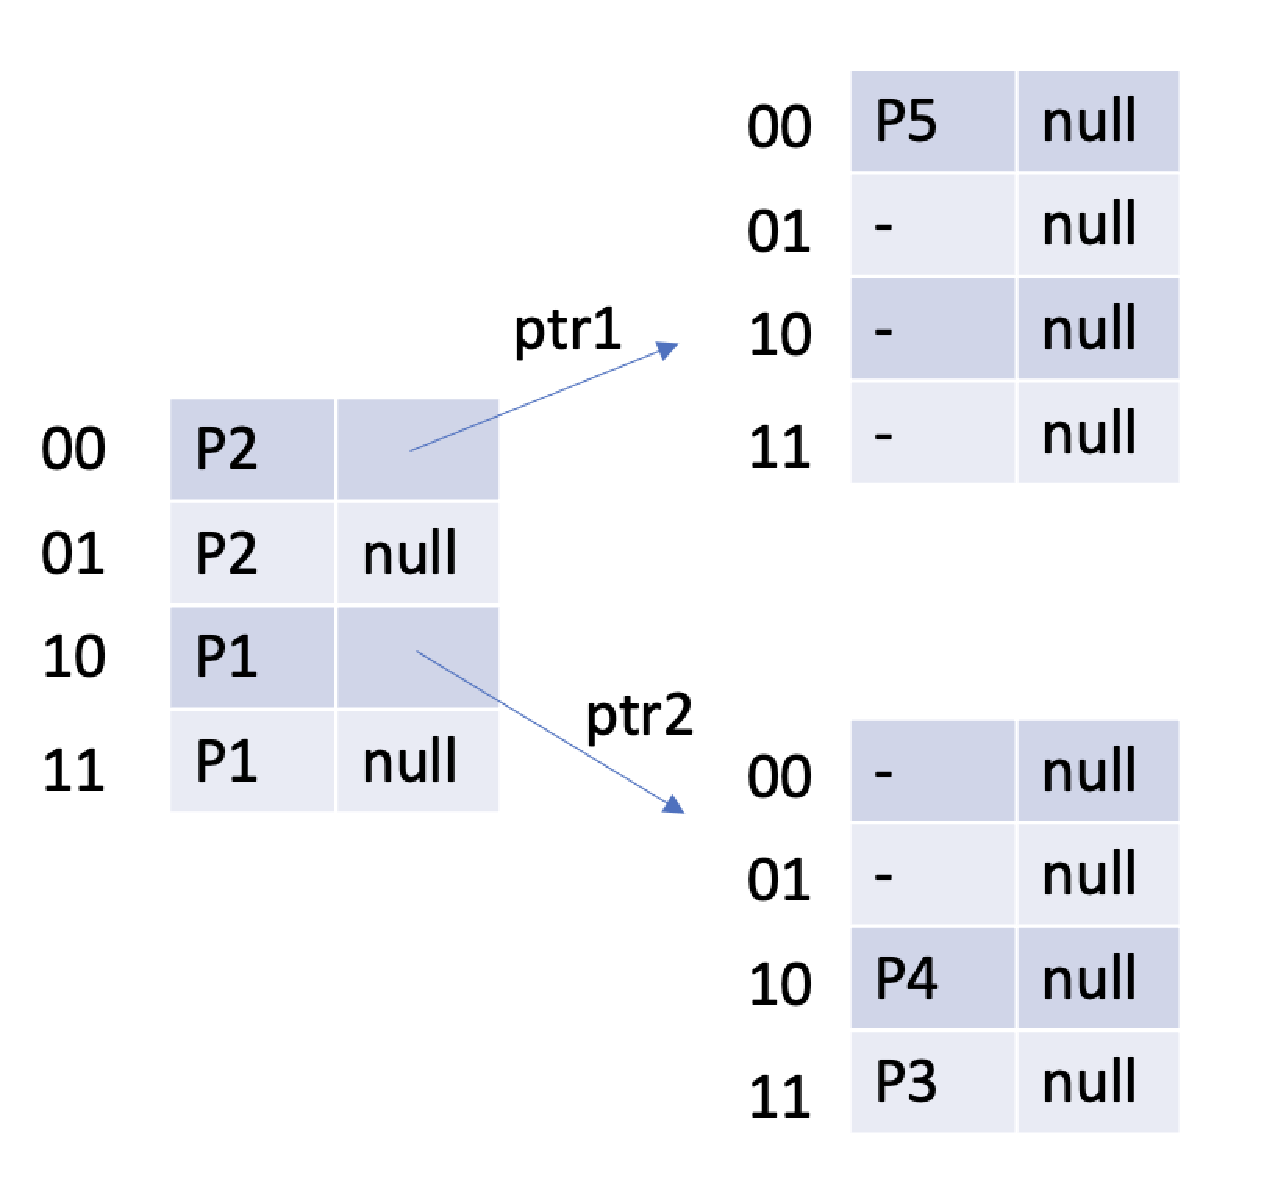
\includegraphics[scale=0.5]{figures/trie_nodes.pdf}
    \label{fig:dvp}
\end{figure}

\end{problem}

\subsection*{Answer 2:}
The answer to this question will be structured from right to left, top to bottom with the enumeration, with both the bit array and the value array being included in each of the enumerations.
\begin{enumerate}
    \item[(a)] Bit: 1111, value: [ptr1, P2, ptr2, P1].
    \item[(b)] Bit: 1100, value: [P5, P2]
    \item[(c)] Bit: 1011, value: [P1, P4, P3]  
\end{enumerate}
\begin{problem}{3: Reading}
Now that we've learned about the Network Layer (IP), let's read about an alternative to IP that is currently in progress. \href{https://named-data.net/techreport/TR001ndn-proj.pdf}{This} technical report explains NDN. Please read through Section 2.2.3 answer the following questions:
\begin{enumerate}
    \item What is one argument for why NDN is better suited for how the internet works today?
    \item What are some challenges in getting widespread use of NDN?
\end{enumerate}
\end{problem}
\subsection*{Answer 3:}
\begin{enumerate}
    \item One argument for why NDN is better suited for how the internet works today is that the namespace for hosts in NDN is unbounded. As we have discussed in class, there is an issue with IPv4 in the sense that we have a bounded number of possible host names which has inspired hacky work arounds, but remains a current limitation to the internet. However, under NDN, we would be able to remedy this as well as discard any future worries we may have about exhausting our library of host names.
    \item Some challenges in getting widespread use of NDN are the facts there are issues with keeping the routing tables in a manageable size while scaling to the number of hosts/multitude of prefixes we may have, a possibly long run-time for variable length name lookups within the routing table, as well as a need to work to combat DNS attacks which would be possible within the network.  
\end{enumerate}
\begin{problem}{4}
How long did this assignment take you?
\end{problem}
\subsection*{Answer 4:}
This assignment took me $\approx 4$ hours.
\begin{problem}{5: Extra (optional) reading}
When we left off in class, we said the Lulea compression helps the reduce memory usage and achieves reasonably fast lookup, but insertion was quite slow. Section 11.8 of the book describes ways of making insertion faster. There is no work or credit or extra credit associated with reading this - just more information if it interests you.
\end{problem}
\end{document}
